\documentclass{article}
\usepackage{graphicx}
\usepackage{amsmath}
\usepackage{xcolor}
\usepackage{subcaption}
\usepackage{algorithm}
\usepackage{algpseudocode}
\usepackage{cite}

\begin{document}

\title{Adapter les GNNs à la classification d'images}
\author{Alexis Vannson}
\date{\today}
\maketitle

\begin{abstract}
Ce document présente une méthode pour adapter les Graph Neural Networks (GNN) à la classification d'images, en détaillant le workflow depuis la conversion des images en graphes jusqu'à la mise à jour des paramètres du modèle. Nous montrons comment le message passing et le pooling global peuvent être utilisés pour améliorer les performances de classification.
\end{abstract}

\tableofcontents
\newpage

\section*{Introduction}
Les CNNs (Convolutional Neural Networks) sont des réseaux de neurones spécialisés dans le traitement des données ayant une structure en grille, comme les images. Ils sont très performants pour la classification d'images mais ne prennent pas pleinement en compte les relations complexes entre pixels éloignés. C'est là qu'interviennent les Graphes Neuraux (GNN), qui permettent aux pixels proches d'échanger des informations, améliorant ainsi la compréhension globale de l'image. Dans ce papier, nous allons analyser le fonctionnement des GNNs et illustrer le workflow qui permet d'obtenir une prédiction à partir d'une image.

\section{Structure en Graphe}
Pour commencer, il faut convertir les images en graphes. Les images en format RGB sont représentées par trois matrices, chacune représentant l'intensité d'une couleur respective. Un graphe est une structure de données composée de nœuds reliés par des arêtes. Notre image représentée par les trois matrices est convertie en un graphe en créant un nœud pour chaque pixel, avec les trois valeurs de couleur à cette position. Cette opération se passe dans la première boîte du workflow (cf. Figure \ref{fig:workflow}).

\begin{figure}[h]
    \centering
    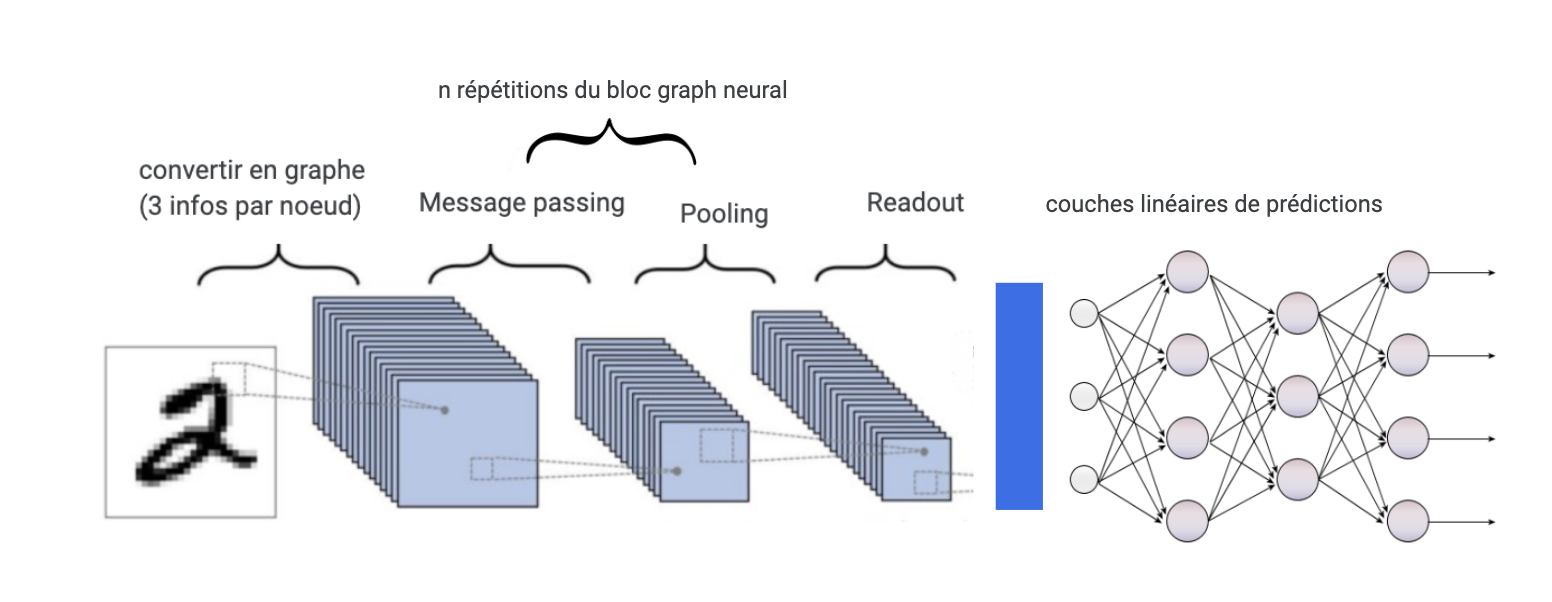
\includegraphics[width=1.2\textwidth]{workflow2.png}
    \caption{Illustration du workflow}
    \label{fig:workflow}
\end{figure}

\begin{figure}[h]
    \centering
    \begin{subfigure}[b]{0.4\textwidth}
        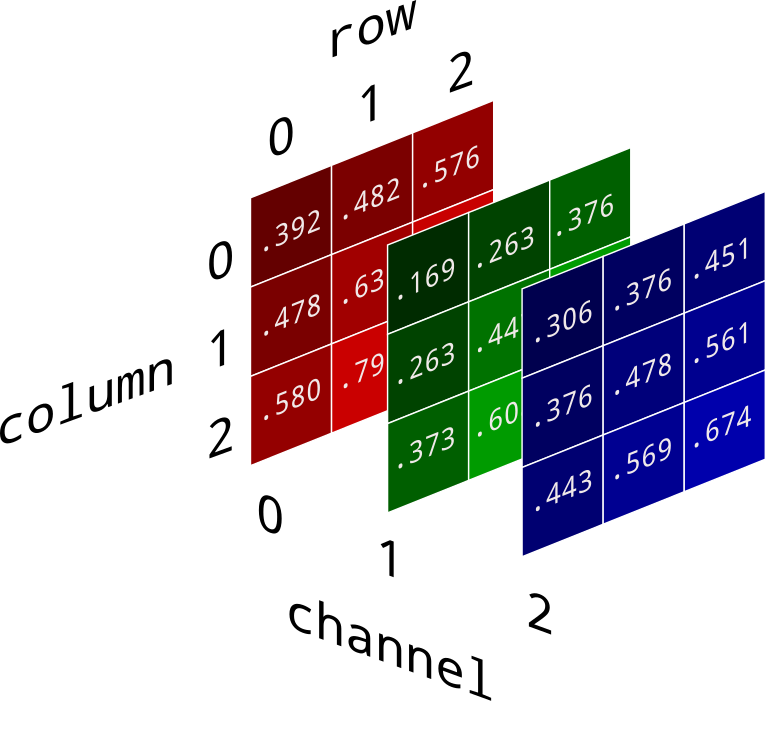
\includegraphics[width=\textwidth]{rgb.png}
        \caption{Représentation initiale de l'image}
        \label{fig:rgb}
    \end{subfigure}
    \hfill
    \begin{subfigure}[b]{0.4\textwidth}
        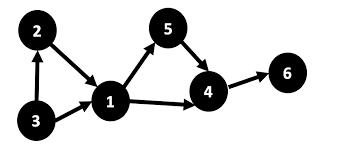
\includegraphics[width=\textwidth]{downloada.png}
        \caption{Représentation du graphe}
        \label{fig:graphe}
    \end{subfigure}
    \caption{Comparaison des différentes étapes de conversion}
    \label{fig:comparison}
\end{figure}

\section{Message Passing}
Une fois l'image convertie en graphe, commence le message passing. Le message passing consiste en un échange d'informations entre les nœuds liés. On obtient ainsi le nouveau nœud enrichi de ses voisins \textcolor{orange}{$h_v^{(k)}$} avec l'expression suivante :
\[
\textcolor{orange}{h_v^{(k)}} = \textcolor{red}{f^{(k)}} \left( \textcolor{teal}{W^{(k)}} \cdot \frac{\sum_{u \in \mathcal{N}(v)} \textcolor{purple}{h_u^{(k-1)}}}{|\mathcal{N}(v)|} + \textcolor{teal}{B^{(k)}} \cdot \textcolor{orange}{h_v^{(k-1)}} \right)
\]

Les caractéristiques des nœuds voisins sont agrégées en calculant la moyenne des caractéristiques des nœuds voisins :
\[
\frac{\sum_{u \in \mathcal{N}(v)} \textcolor{purple}{h_u^{(k-1)}}}{|\mathcal{N}(v)|}
\]

Cette agrégation est pondérée par la matrice de poids \textcolor{teal}{$W^{(k)}$} qui détermine l'importance relative de chaque caractéristique. Ensuite, on ajoute les caractéristiques initiales du nœud pondérées par un poids \textcolor{teal}{$B^{(k)}$} \(\cdot\) \textcolor{orange}{$h_v^{(k-1)}$}. Finalement, on passe le résultat de ces opérations dans une fonction non linéaire \textcolor{red}{$f^{(k)}$}, ce qui permet de ne pas être limité aux problèmes linéaires.



On peut visualiser le bloc Graph Neural avec le graphique ci-dessus où les boules vertes représentent les nœuds voisins qui sont agrégés en prenant en compte le poids de la matrice \textcolor{teal}{$W^{(k)}$} (représenté par w1, w2, w3) et le biais \textcolor{teal}{$B^{(k)}$} \(\cdot\) \textcolor{orange}{$h_v^{(k-1)}$} (b1 sur le graphique), puis passent dans la fonction d'activation \textcolor{red}{$f^{(k)}$} (g sur le graphique).

\begin{figure}[h]
    \centering
    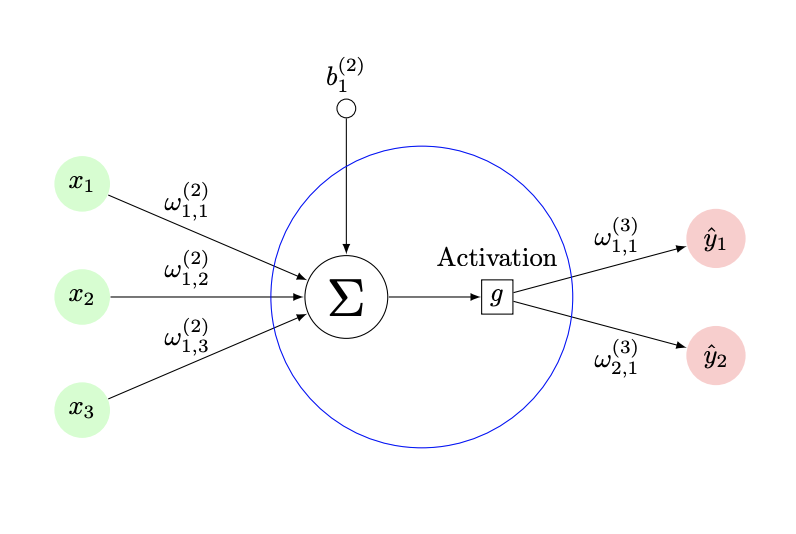
\includegraphics[width=0.6\textwidth]{v.png}
    \caption{Illustration d'un Bloc Graph Neural}
    \label{fig:bloc}
\end{figure}

\section{Boucle d’Entraînement}

\subsection{Bloc Graph Neural}
Après avoir converti l'image initiale en graphe, l’entraînement commence avec un enchaînement de blocs Graphs neuraux. Les blocs Graphs neuraux sont constitués de couches de message passing, qui viennent d’être définies, avec des couches de Pooling. Ces couches de Pooling vont identifier les nœuds les plus importants pour la bonne compréhension du graphe en leur attribuant tous un score grâce à un MLP (comme détaillé ci-dessous). Nous allons alors sélectionner les K meilleurs nœuds (effacer les autres) pour éliminer le bruit et diminuer la charge computationnelle.

\[
\text{score}(v_i) = W_2 \sigma(W_1 h_i + b_1) + b_2
\]

Avec :
\begin{align*}
W_1 & : \text{Matrice de poids pour la première couche cachée} \\
b_1 & : \text{Vecteur de biais pour la première couche cachée} \\
\sigma & : \text{Fonction d'activation (par exemple, ReLU)} \\
W_2 & : \text{Matrice de poids pour la couche de sortie} \\
b_2 & : \text{Vecteur de biais pour la couche de sortie}
\end{align*}

\subsection{Readout}
Ensuite, plusieurs itérations de blocs Graph Neural plus tard, nous allons synthétiser les nœuds du graphe en un vecteur grâce au global Pooling, aussi appelé Readout. Pour cela, nous allons prendre la moyenne, le maximum ou la somme des caractéristiques de chaque nœud (une méthode hybride ou un mécanisme d’attention sont également possibles) pour obtenir un vecteur. Cette étape est illustrée par le rectangle bleu dans le workflow. De là, le vecteur va être passé dans des couches linéaires de classification (comme dans un CNN classique) pour obtenir une probabilité finale pour chaque classe (illustré par les nœuds à droite du Readout dans le workflow).

\subsection{Loss}
Une fois les prédictions effectuées, nous allons estimer la qualité de celles-ci avec une fonction loss, qui va représenter la distance des prédictions à la réalité à travers une valeur. Dans le cas où nous avons deux classes, la Binary Cross Entropy Loss (BCE) est performante.

\[
\text{BCE} = -\frac{1}{N} \sum_{i=0}^{N} \left( y_i \cdot \log(\hat{y}_i) + (1 - y_i) \cdot \log(1 - \hat{y}_i) \right)
\]

\begin{itemize}
    \item \( N \) : Nombre total d'échantillons.
    \item \( y_i \) : Véritable étiquette de la classe (0 ou 1) pour l'échantillon \( i \).
    \item \( \hat{y}_i \) : Probabilité prédite que l'échantillon \( i \) appartienne à la classe 1.
\end{itemize}

\subsection{Fonctionnement}
\begin{itemize}
    \item Lorsque \( y_i = 1 \) : La BCE pénalise fortement si \( \hat{y}_i \) est proche de 0 (mauvaise prédiction) car \( \log(\hat{y}_i) \) tend vers \( -\infty \) lorsque \( \hat{y}_i \) tend vers 0.
    \item Lorsque \( y_i = 0 \) : La BCE pénalise fortement si \( \hat{y}_i \) est proche de 1 (mauvaise prédiction) car \( \log(1 - \hat{y}_i) \) tend vers \( -\infty \) lorsque \( \hat{y}_i \) tend vers 1.
\end{itemize}

\section{Backpropagation}
\subsection*{Calcul des Gradients}
Les gradients de la perte sont calculés par rapport à chaque paramètre du modèle en utilisant la règle de la chaîne, qui permet de décomposer le gradient d'une fonction composée en un produit de gradients plus simples. Cela permet de déterminer l'influence de chaque poids sur la perte.

Par exemple, pour un poids \( w \) dans le modèle, le gradient de la perte par rapport à ce poids est noté \( \frac{\partial L}{\partial w} \). Ce gradient indique la direction et l'ampleur du changement nécessaire pour réduire la perte.

La règle de la chaîne est exprimée mathématiquement par la formule suivante :

\[
\frac{\partial L}{\partial w} = \frac{\partial L}{\partial y} \cdot \frac{\partial y}{\partial w}
\]

où \( y \) est une variable intermédiaire qui dépend du poids \( w \).

\subsection*{Mise à Jour des Paramètres}
Une fois les gradients calculés, les paramètres du modèle sont mis à jour pour minimiser la fonction de perte. La mise à jour des paramètres se fait généralement selon l'algorithme de descente de gradient :

\begin{itemize}
    \item \( a_n \) représente les paramètres actuels du modèle à l'itération \( n \).
    \item \( \lambda \) est le taux d'apprentissage, un hyperparamètre qui contrôle la taille des pas de mise à jour.
    \item \( \nabla P \) est le gradient de la fonction de perte par rapport aux paramètres.
    \item La mise à jour est effectuée comme suit : \( a_{n+1} = a_n - \lambda \nabla P \).
    \item Cela signifie que chaque poids \( w \) est ajusté de la manière suivante :
    \[
    w_{n+1} = w_n - \lambda \frac{\partial L}{\partial w}
    \]
    où \( w_n \) est la valeur actuelle du poids, \( \frac{\partial L}{\partial w} \) est le gradient de la perte par rapport à ce poids, et \( \lambda \) est le taux d'apprentissage.
    \item En répétant ce processus sur plusieurs itérations, les poids sont ajustés pour minimiser la perte, entraînant ainsi le modèle.
\end{itemize}
\section{Pseudo-code de l'Algorithme}
\begin{algorithm}
\caption{Entraînement des Graph Neural Networks}
\begin{algorithmic}[1]
    \State \textbf{Input:} Graph $G = (V, E)$, initial node features $h_v^{(0)}$
    \State \textbf{Parameters:} Learning rate $\lambda$, Number of iterations $T$
    \For{each iteration $t = 1$ to $T$}
        \For{each layer $k = 1$ to $K$}
            \For{each node $v \in V$}
                \State $h_v^{(k)} \leftarrow f^{(k)} \left( W^{(k)} \cdot \frac{\sum_{u \in \mathcal{N}(v)} h_u^{(k-1)}}{|\mathcal{N}(v)|} + B^{(k)} \cdot h_v^{(k-1)} \right)$
            \EndFor
            \State $h^{(k)} \leftarrow \text{Pooling}(h^{(k)})$ \Comment{Pooling step}
        \EndFor
        \State $Z \leftarrow \text{Readout}(h^{(K)})$ \Comment{Readout step}
        \State $\hat{y} \leftarrow \text{LinearClassifier}(Z)$ \Comment{Classification step}
        \State $L \leftarrow \text{BinaryCrossEntropyLoss}(y, \hat{y})$ \Comment{Loss computation}
        \For{each parameter $w$}
            \State $\frac{\partial L}{\partial w} \leftarrow \text{ComputeGradient}(L, w)$ \Comment{Gradient computation}
            \State $w \leftarrow w - \lambda \frac{\partial L}{\partial w}$ \Comment{Update parameter}
        \EndFor
    \EndFor
    \State \textbf{Output:} Trained parameters $W, B$
\end{algorithmic}
\end{algorithm}

\section*{Conclusion}
Nous avons démontré comment les GNNs peuvent être utilisés pour la classification d'images en exploitant les relations locales et globales entre les pixels. 


\end{document}
